% ============================================================
% Oppgave 6
% ============================================================
\hypertarget{oppgave6}{}
\section*{Oppgave 6}
\addcontentsline{toc}{section}{Oppgave 6}
\subsection*{a)}
Filterkoeffisientene samles i vektoren:
\begin{verbatim}
b = [0.02 0.04 0.08 0.12 0.15 0.16 ...
     0.15 0.12 0.08 0.04 0.02];
\end{verbatim}
Koeffisientene er symmetriske omkring den midterste koeffisienten. Dette gir da en vektet gjennomsnittseffekt, hvor midterste koeffisient har størst vekt, og koeffisientene avtar symmetrisk mot kantene.
\subsection*{b)}
Filteret inneholder koeffisientene:
\[
b_0,b_1,\ldots,b_{10}
\]
Den største forsinkelsen er derfor:
\[
x[n-10]
\]
Filterordenen er dermed:
\[
\boxed{10}
\]
Den diskrete sinussekvensen er:
\[
x[n]
=
\sin(0.0625\pi n)
\]
for:
\[
n=0,\ldots,63
\]
I Octave genereres og filtreres signalet med:
\begin{verbatim}
n = 0:63;
b = [0.02 0.04 0.08 0.12 0.15 0.16 ...
     0.15 0.12 0.08 0.04 0.02];
x0625 = sin(0.0625*pi*n);
y0625 = filter(b, 1, x0625);
figure;
hold on;
stem(n, x0625, "b");
stem(n, y0625, "r");
hold off;
grid on;
legend("Innsignal", "Utsignal");
xlabel("n");
ylabel("Amplitude");
\end{verbatim}
\subsection*{c)}
Amplituderesponsen til FIR-filteret ved:
\[
\hat{\omega}
=
0.0625\pi
\]
kan finnes fra ved å ta absoluttverdien av frekvensresponsen:
\[
H(e^{j\omega})
=
\sum_{n=0}^{10}
b_n z^{-n}, \quad \text{hvor } z = e^{j\omega}
\]
\[
    |H(e^{j\omega})| = \left|\sum_{n=0}^{10} b_n e^{-j\omega n}\right|
\]
For:
\[
\omega
=
0.0625\pi
\]
får vi:
\[
|H(e^{j0.0625\pi})|
\approx
0.8878
\]
Innsignalet har amplitude:
\[
A_{\mathrm{inn}}=1
\]
mens utsignalet etter oppstartstransienten (oppstartperioden hvor forsinkelses leddene ikke er fylt opp) har amplitude omtrent:
\[
A_{\mathrm{ut}}
\approx
0.888
\]
Amplituden til utsignalet er dermed omtrent:
\[
\boxed{
88.8\%
}
\]
av amplituden til innsignalet. Filteret demper altså denne
frekvenskomponenten med omtrent:
\[
100\%-88.8\%
=
11.2\%
\]
Dette ser vi tydelig i figuren under:
\begin{figure}[H]
\centering
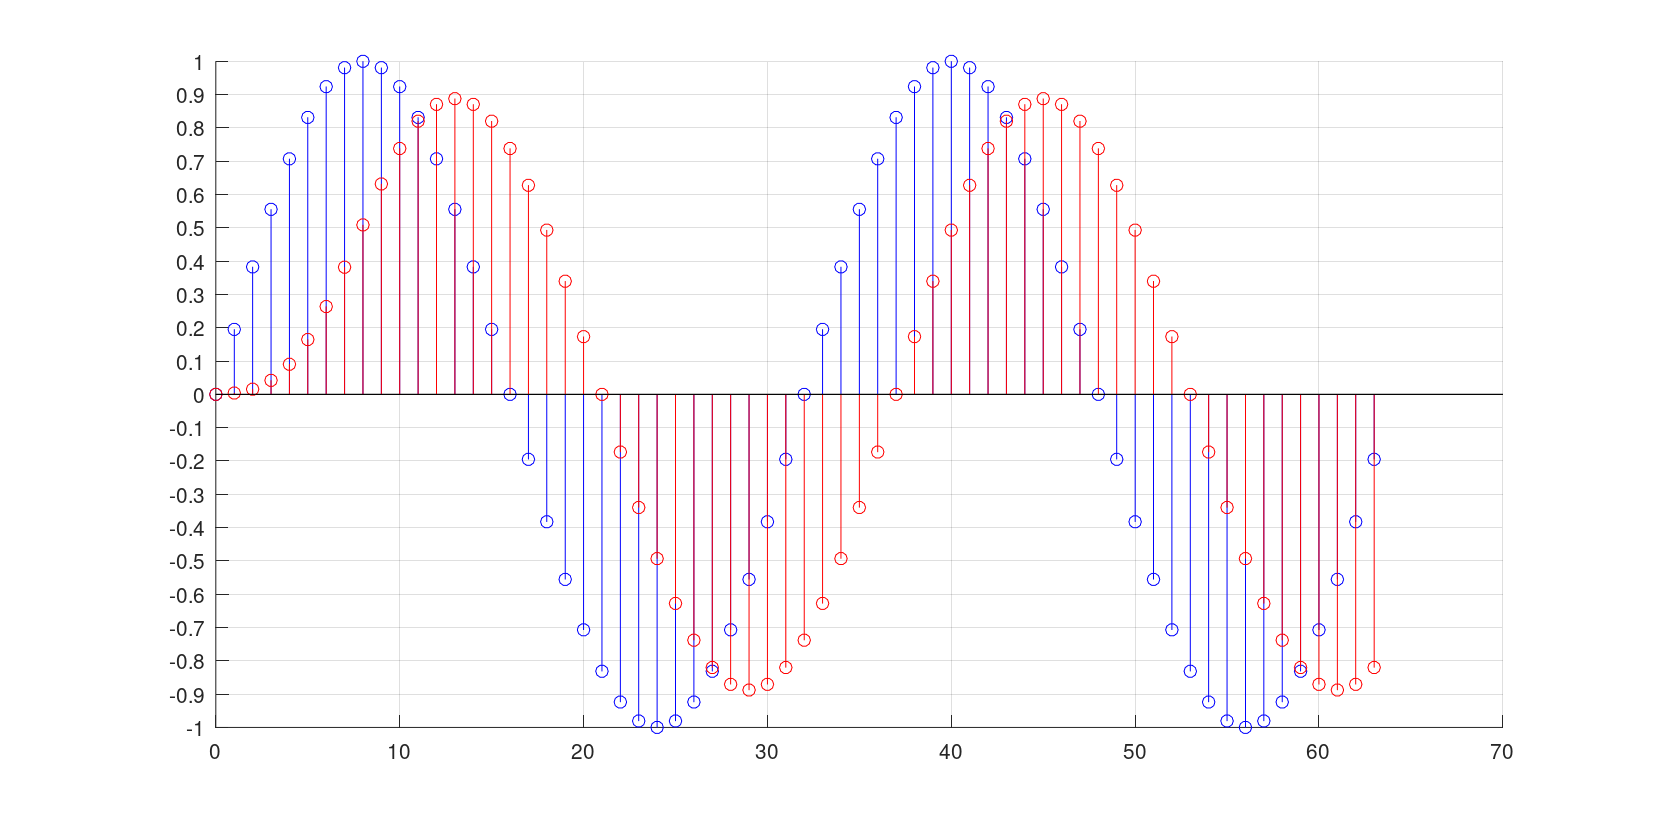
\includegraphics[width=1\textwidth]{Media/opp6.png}
\caption{Innsignal og utsignal for FIR-filteret.}
\end{figure}
